\documentclass[10pt,letterpaper,oneside]{article}

\usepackage{multirow}
\usepackage{makecell}

\usepackage{lscape}
\usepackage{pdflscape}

% The file intend to keep track of good practices in Latex writing.

%==============================
% DOCUMENT
%==============================

% Fix some error reporting
\vfuzz2pt % Don't report over-full v-boxes if over-edge is small
\hfuzz2pt % Don't report over-full h-boxes if over-edge is small

% All the same, there are commands, classes and packages which are outdated and superseded. 
% nag provides routines to warn the user about the use of those.
\usepackage[l2tabu,orthodox]{nag}

%==============================
% BIBLIOGRAPHY
%==============================

% \addbibresource{references.bib} % in your preamble
% \citet{key}, \citep{key} % in the document
% \printbibliography % to generate the reference section
\usepackage[
backend=bibtex8, 
style=ieee, 
sorting=none, 
natbib=true, 
doi=false, 
isbn=false, 
url=false, 
eprint=false, 
maxcitenames=1, 
mincitenames=1
]{biblatex}

%==============================
% TEXT
%==============================

% \autoref{key} % instead of Figure~\ref{key}, Table~\ref{key}, Equation~\ref{key}, or Section~\ref{key}
\usepackage[pdftex,colorlinks]{hyperref}
% fix names for autoref
\def\sectionautorefname{Section}
\def\subsectionautorefname{Section}
\newcommand*{\Appendixautorefname}{Appendix}

% \acrodef{ICP}{Iterative Closest Point} % in the preamble
% \ac{ICP} % in the document
\usepackage[printonlyused]{acronym}

% International unit system 
% e.g., \SI{1000}{\m\squared}, \num{20000}
\usepackage{siunitx}
\sisetup{group-separator = \text{\,}} % small space for thousand separator

% avoid single line on a page or single line under a figure
% no command to use
\usepackage[all]{nowidow}

% Colored text
\usepackage[dvipsnames]{xcolor}

% Fill the template with text
\usepackage{lipsum}

% Better command to make sure that people don't confuse lipsum text with real text
\newcommand{\lightlipsum}[1][0]{\textcolor{gray!50}{\lipsum[#1]}}

%==============================
% FIGURE
%==============================

% Preferred figure format:
% - pdf or eps for graphs and schemas
% - jpg for photo
% Don't use png as each compilation decompress the image, thus making compilation time
% untolerable when there are more than 5 images...

% \includegraphics[width=\textwidth]{filename}
\usepackage[pdftex]{graphicx}

% convert eps to pdf, you need to skip the file extension to work properly
% \includegraphics{filename} % instead of \includegraphics{filename.eps}
\usepackage{epstopdf}

% for Inkscape figures, import tex files in other folder and keep paths coherent
% e.g., \import{images}{timeline.pdf_tex}
\usepackage{import}

% include path for logos
\graphicspath{{./latexGoodPractices/}}

%==============================
% TABLE
%==============================

% Cleaner spacing for tables
% \toprule, \midrule, \bottomrule % instead of \hline
\usepackage{booktabs}

% Tables that can fit page length
% e.g.,three columns with the second one being twice as large as the others
% \begin{tabu}{X X[2] X}
\usepackage{tabu}

%==============================
% MATH
%==============================

% Better symboles
\usepackage{amssymb,amsfonts,amsmath,amscd}

% \bm % in equations for proper bold font
\usepackage{bm} 

% Some handy commands
\newcommand{\norm}[1]{\left\Vert#1\right\Vert}
\newcommand{\abs}[1]{\left\vert#1\right\vert}
\newcommand{\set}[1]{\left\{#1\right\}}
\newcommand{\Real}{\mathbb R}
\newcommand{\bbm}{\begin{bmatrix}}
\newcommand{\ebm}{\end{bmatrix}}




%==============================================================
% FILL THIS SECTION

\newcommand{\reportTitle}{Theodolite notice of use}
\newcommand{\reportAuthors}{Maxime Vaidis}
\newcommand{\reportDate}{\today} % or manually: November 23, 2017

\newcommand{\reportVersions}{
1.0 & \today & Initial writing %\\
%1.0 & November 23, 2017 & Final writing
}
% Change to your specific bibliography file
\addbibresource{./references.bib}
%==============================================================

\usepackage{chemist}
\newcommand{\ie}{i.e., }
\newcommand{\eg}{i.e., }
% Use subcaption package
\usepackage{subcaption}

%\acrodef{DARPA}{Defense Advanced Research Projects Agency}

% ---------------------------------------------------------------
% Load style
%----------------------------------------
% Page style

% Set the page size
\addtolength{\hoffset}{-1.0in} \addtolength{\voffset}{-0.75in}
\setlength{\textwidth}{6.75in} \setlength{\textheight}{8.25in}
\setlength{\headheight}{0.6in}
\setlength{\headsep}{0.2in}

\setlength{\footskip}{40pt}
\setlength{\fboxsep}{12pt}

% Set the paragraph skip
\setlength{\parskip}{3pt}

% Access to a counter for the number of pages
\usepackage{lastpage}

% To allow text justify on the right
\usepackage{ragged2e}

%----------------------------------------
% Title style

\newcommand{\makeCustomTitle}
{
\begin{center}
\LARGE{\textbf{\reportTitle{}}}
\\
\vspace{5pt}
\normalsize{\reportAuthors{}}
\\
\reportDate{}
\end{center}
\begin{flushright}
\footnotesize{
\begin{tabu}{ccX}
\toprule
\emph{Version} & \emph{Date} & \emph{Comments} \\
\midrule
\reportVersions{} \\
\bottomrule
\end{tabu}
}
\end{flushright}
}

%----------------------------------------
% Section style
\usepackage{sectsty}

% Set the section labeling font
\allsectionsfont{\textsf\bfseries}

%----------------------------------------
% Caption style
\usepackage[font=small, labelfont=bf, skip=5pt]{caption}

%----------------------------------------
% header style
\usepackage{fancyhdr}



% Define the title page style
\fancypagestyle{titlePage}{%
\fancyhf{}%

\fancyhead[L]{
\includegraphics[height=0.45in]{UL_N}}
\fancyhead[C]{\raisebox{0.2in}{\textsc{Technical Report}}}
\fancyhead[R]{
\includegraphics[height=0.45in]{norlab_logo_acronym_dark}}
\fancyfoot[C]{\thepage/\pageref*{LastPage}}

\renewcommand{\headrulewidth}{0.1pt}
\renewcommand{\footrulewidth}{0.2pt}
}

% Define the page style for the other pages
\fancypagestyle{plain}{%
\fancyhf{}
\fancyhead[L]{\reportTitle{}}
\fancyfoot[C]{\thepage/\pageref*{LastPage}}
\renewcommand{\headrulewidth}{0.1pt}
\renewcommand{\footrulewidth}{0.1pt}
}

% Set the page style for all the document except the first page
\pagestyle{plain}

%----------------------------------------
% footnote style
\usepackage{fnpos}
% Fix the footnotes location
\makeFNbottom \makeFNbelow

% ---------------------------------------------------------------
% Author

\author{\reportAuthors{} \\
       Laval University\\
       1065, av. de la Médecine \\
       Quebec, Qc \\
       Canada G1V 0A6 \\
}

% ---------------------------------------------------------------
% PDF setup
\hypersetup{%
    pdftitle={\reportTitle},
    pdfauthor={\@author},
    pdfkeywords={research, project, robotics, norlab, Northern Robotics Lab, Master's},
    pdfsubject={},
    pdfstartview={},
    urlcolor=cyan,
    linkcolor=red,
}%
% ---------------------------------------------------------------


% Add your other packages here
% make sure to check prembule.tex first!


%================================================================
\begin{document}
\makeCustomTitle
\thispagestyle{titlePage}

% ---------------------------------------------------------------
\section{Introduction}

En robotique mobile, il peut être important d'avoir des données de référence afin de comparer et valider les résultats obtenus par un algorithme.
Cette comparaison est d'autant plus importante pour évaluer la localisation d'une plateforme mobile.
En effet, les capteurs tels que les GPS ont une imprécision pouvant être de plusieurs mètres et ne peuvent pas être une source fiable pour évaluer finement un algorithme de localisation.
Les algorithmes tels que ICP sont plus précis, mais possèdent des biais sur le long termes qui faussent la localisation.

Pour palier ce problème d'imprécision des mesures, certains corps de métiers comme les topographes ou les géomètre ont recours à des appareils appelés théodolite.
Un théodolite est un instrument de géodésie complété d’un instrument d'optique, qui permet de mesurer des angles dans les deux plans horizontaux et verticaux afin de déterminer une direction.
Ces appareils peuvent également mesurer la distance d'une cible par rapport à eux.
Leur précision angulaire est inférieur au millième de degré, et la précision de la mesure de distance est de l'ordre du millimètre.

De ce fait, il est possible d'obtenir un relevé très précis de n'importe quels objets ciblés.
En plaçant différentes cibles sur un robot mobile, nous pourrions alors obtenir sa pose complète de référence.
Ces données de référence peuvent alors nous servir à évaluer la précision d'ICP et quantifier son biais dans le temps. 

% -------------------------------------------------------------
\section{Equipements}

Afin d'effectuer nos relevés, nous aurons besoin de plusieurs équipements en plus du théodolite.
Il s'agit de moyens de communication entre le théodolite et la plateforme d'acquisition des données, mais également des différents cibles utilisés pour mesurer la distance avec précision.
Ces différents équipements sont présentés dans cette section.

\subsection{Theodolite}

Dans cette section, une description précise du théodolite sera donné, ainsi que l'explication de sa mise en marche pour la prise de mesure.
Le théodolite que nous utilisons est une Station Totale Trimble S7, montré à la \autoref{fig:trimbleS7}.

\begin{figure}[htb]
	\centering
	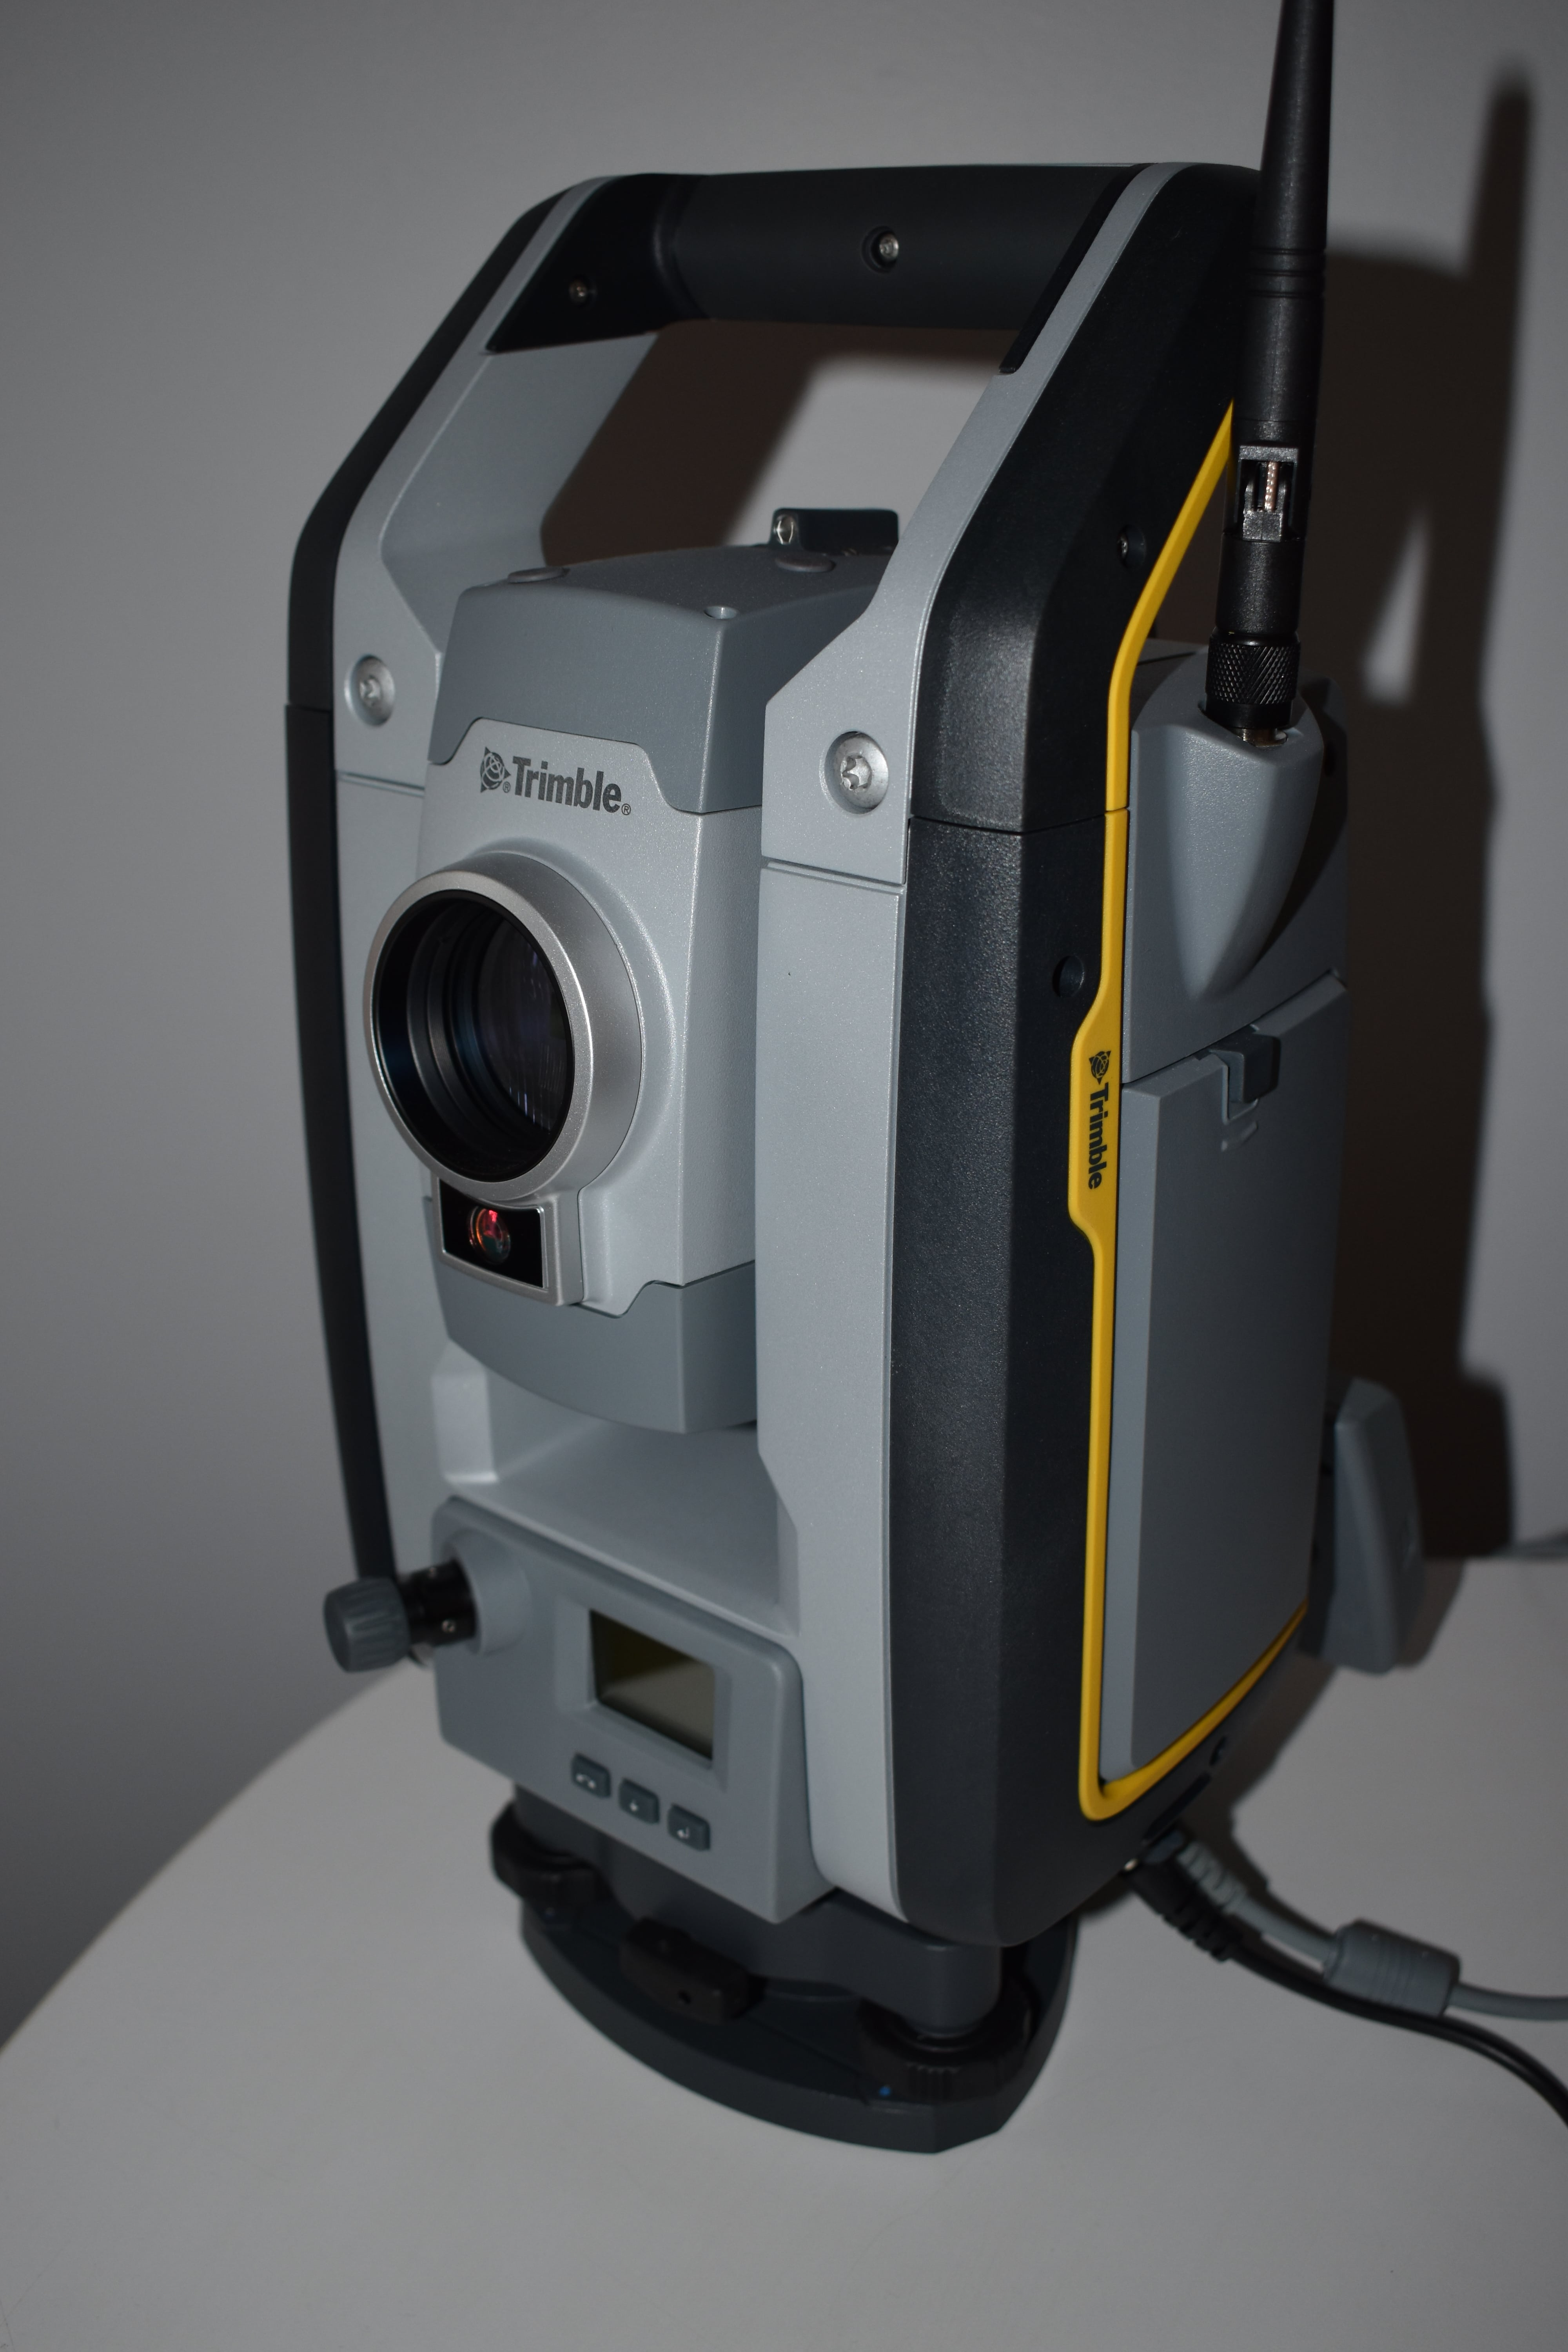
\includegraphics[width=0.2\textwidth]{./figs/trimbleS7.JPG}
	\caption{Trimble S7 of the laboratory.}
	\label{fig:trimbleS7}
\end{figure}

La fiche technique de ce modèle de théodolite est donné dans ce \href{run:S7_DS_french.pdf}{Technical Guide French} ou dans ce \href{run:S7_DS_english.pdf}{Technical Guide English}.
Une courte description des capacités du théodolite y est donné.
La précision et la performance des différents capteurs y sont renseignées, ainsi que la durée des batteries.

Un guide de démarrage rapide de ce modèle est également donné dans ce \href{run:Quick_Start_Guide_French.pdf}{Quick Start Guide French} ou dans ce \href{run:Quick_Start_Guide_English.pdf}{Quick Start Guide English}.
Dans ce guide, une description des équipements du théodolite y est donné.
La première prise en main des équipements y est également expliquée afin de mettre en marche le théodolite pour la prise de mesure.

Avec ce theodolite, d'autres accessoires utiles peuvent être utilisés.
Le laboratoire possède une tablette numérique pouvant être fixé sur le théodolite, montré à \autoref{fig:tablet}.

\begin{figure}[htb]
	\centering
	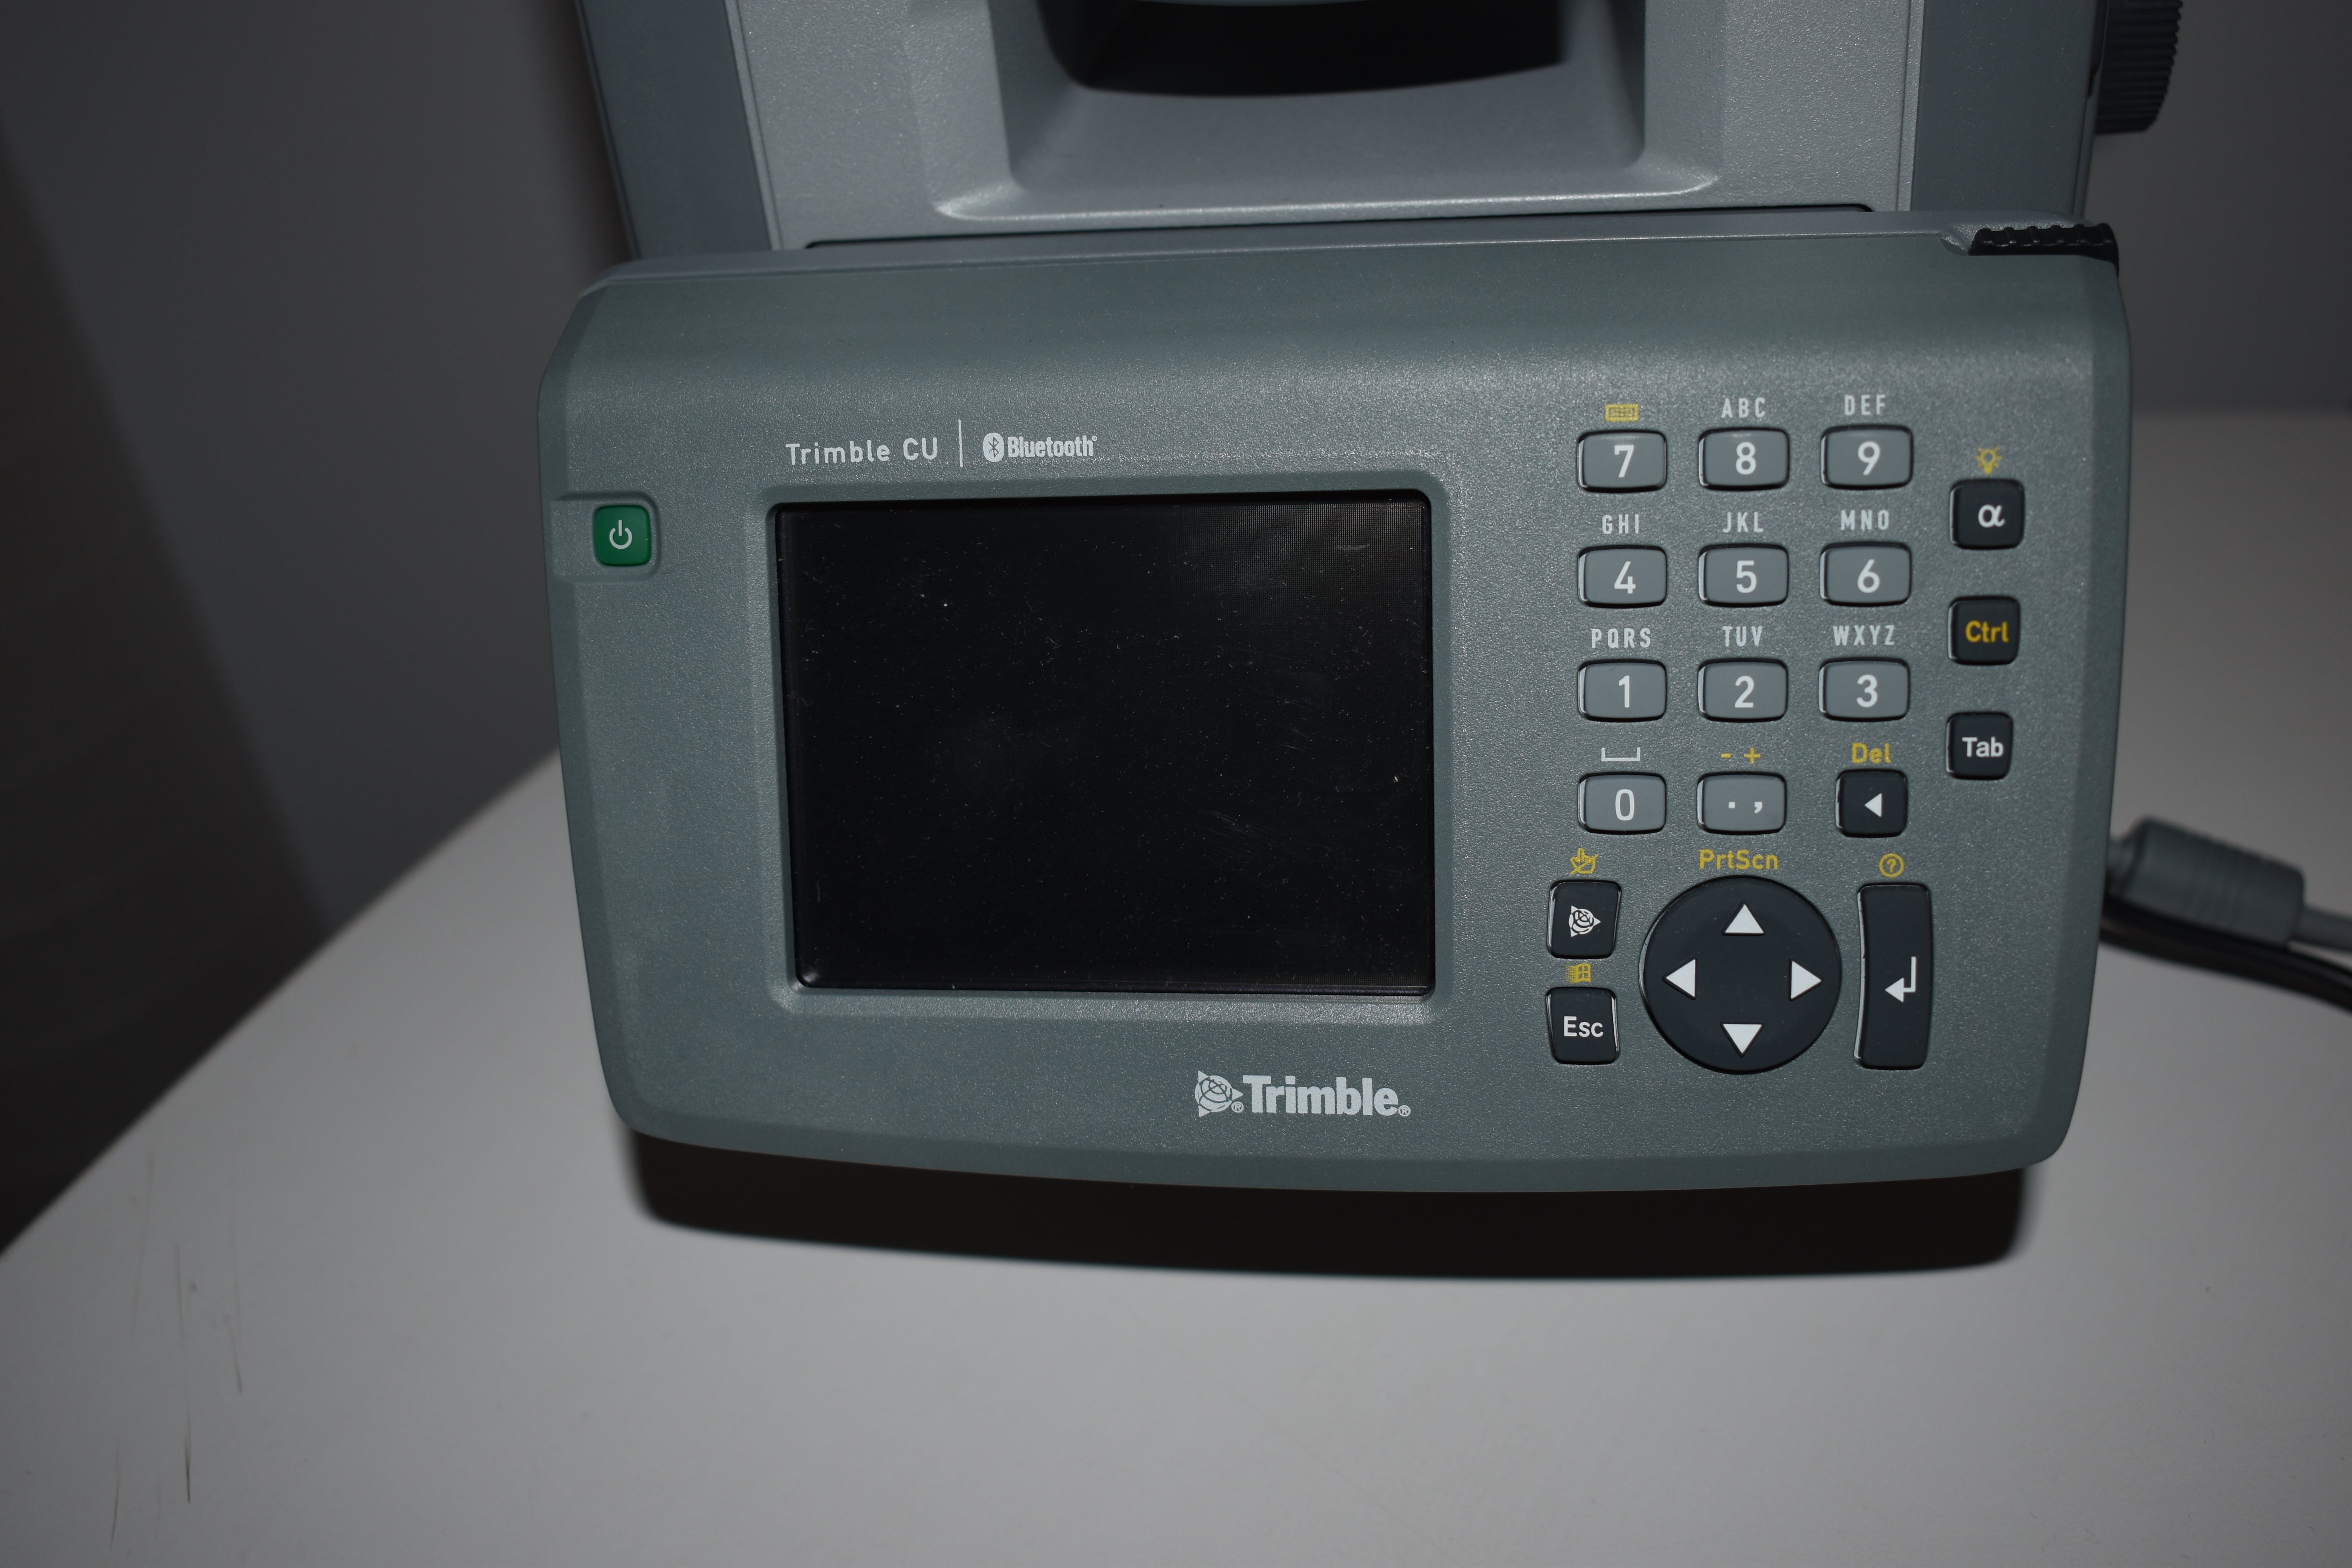
\includegraphics[width=0.3\textwidth]{./figs/Tablet.JPG}
	\caption{Tablet fixed on the trimble S7.}
	\label{fig:tablet}
\end{figure}

Cette tablette possède un OS windows avec le logiciel Trimble Access qui permet de communiquer des commandes au théodolite.
Une desciption détaillée de ce logiciel sera donnée dans la \autoref{sec:software}.
Le théodolite peut prendre en compte différent moyens de communication: Bluetooth, Radio et USB.
Le mode Bluetooth peut être direct (ordinateur vers théodolite via l'application Trimble Access).
Ce mode Bluetooth peut aussi être utilisé pour une communication indirect vers le théodolite.
Dans ce cas, il faut utiliser un relai Trimble TDL 2.4 qui assurera la liaison entre l'ordinateur et le théodolite.
L'ordinateur doit se connecter à ce relai par Bluetooth via l'application Trimble Access. 
Par la suite, le relai va communiquer par radio avec le théodolite, ce qui permet de pouvoir le contrôler à distance (jusqu'à environ 600m).
Le dernier mode de communication est par USB.
C'est celui que l'on va utiliser principalement par la suite.
Tout ces moyens de communication seront décrit en détail avec la présentation du logiciel Trimble Access dans la \autoref{sec:software}.

\subsection{Target}

Afin d'effectuer des mesures, le théodolite a besoin d'une cible.
Ces cibles peuvent être de différent types.
La plus commune est la cible sur papier réfléchissant (reflective foil).
La figure ... en montre quelques exemples.

%%Figure cibles réfléchissantes
%%%%%%%%%%%%%%%%%%%%%%%%%%%%%%%
%%%%%%%%%%%%%%%%%%%%%%%%%%%%%%%
%%%%%%%%%%%%%%%%%%%%%%%%%%%%%%%
%%%%%%%%%%%%%%%%%%%%%%%%%%%%%%%
%%%%%%%%%%%%%%%%%%%%%%%%%%%%%%%
%%%%%%%%%%%%%%%%%%%%%%%%%%%%%%%

Ces cibles sont fournies avec le théodolite et peuvent être placé sur n'importe quels objets.
Cependant le théodolite ne peut mesurer qu'une cible à la fois.
Le théodolite ne fait pas de distinction entre ces différentes cibles réfléchissantes. 
Ainsi, s'il en détecte une nouvelle à proximité d'une autre cible, il peut changer de cible à mesurer automatiquement.
De plus, d'après la fiche technique de la section précédente les performances sont moindres avec ce type de cible (distance et précision réduites).
C'est pourquoi on préférera plutôt les utiliser pour calibrer le théodolite sur des distances courtes, plutôt que de les utiliser pour des prises de mesures lointaine. 

La cible que l'on va utilisé le plus souvent pour traquer notre plateforme robotique est un prisme, montré à la \autoref{fig:prism}.

\begin{figure}[htb]
	\centering
	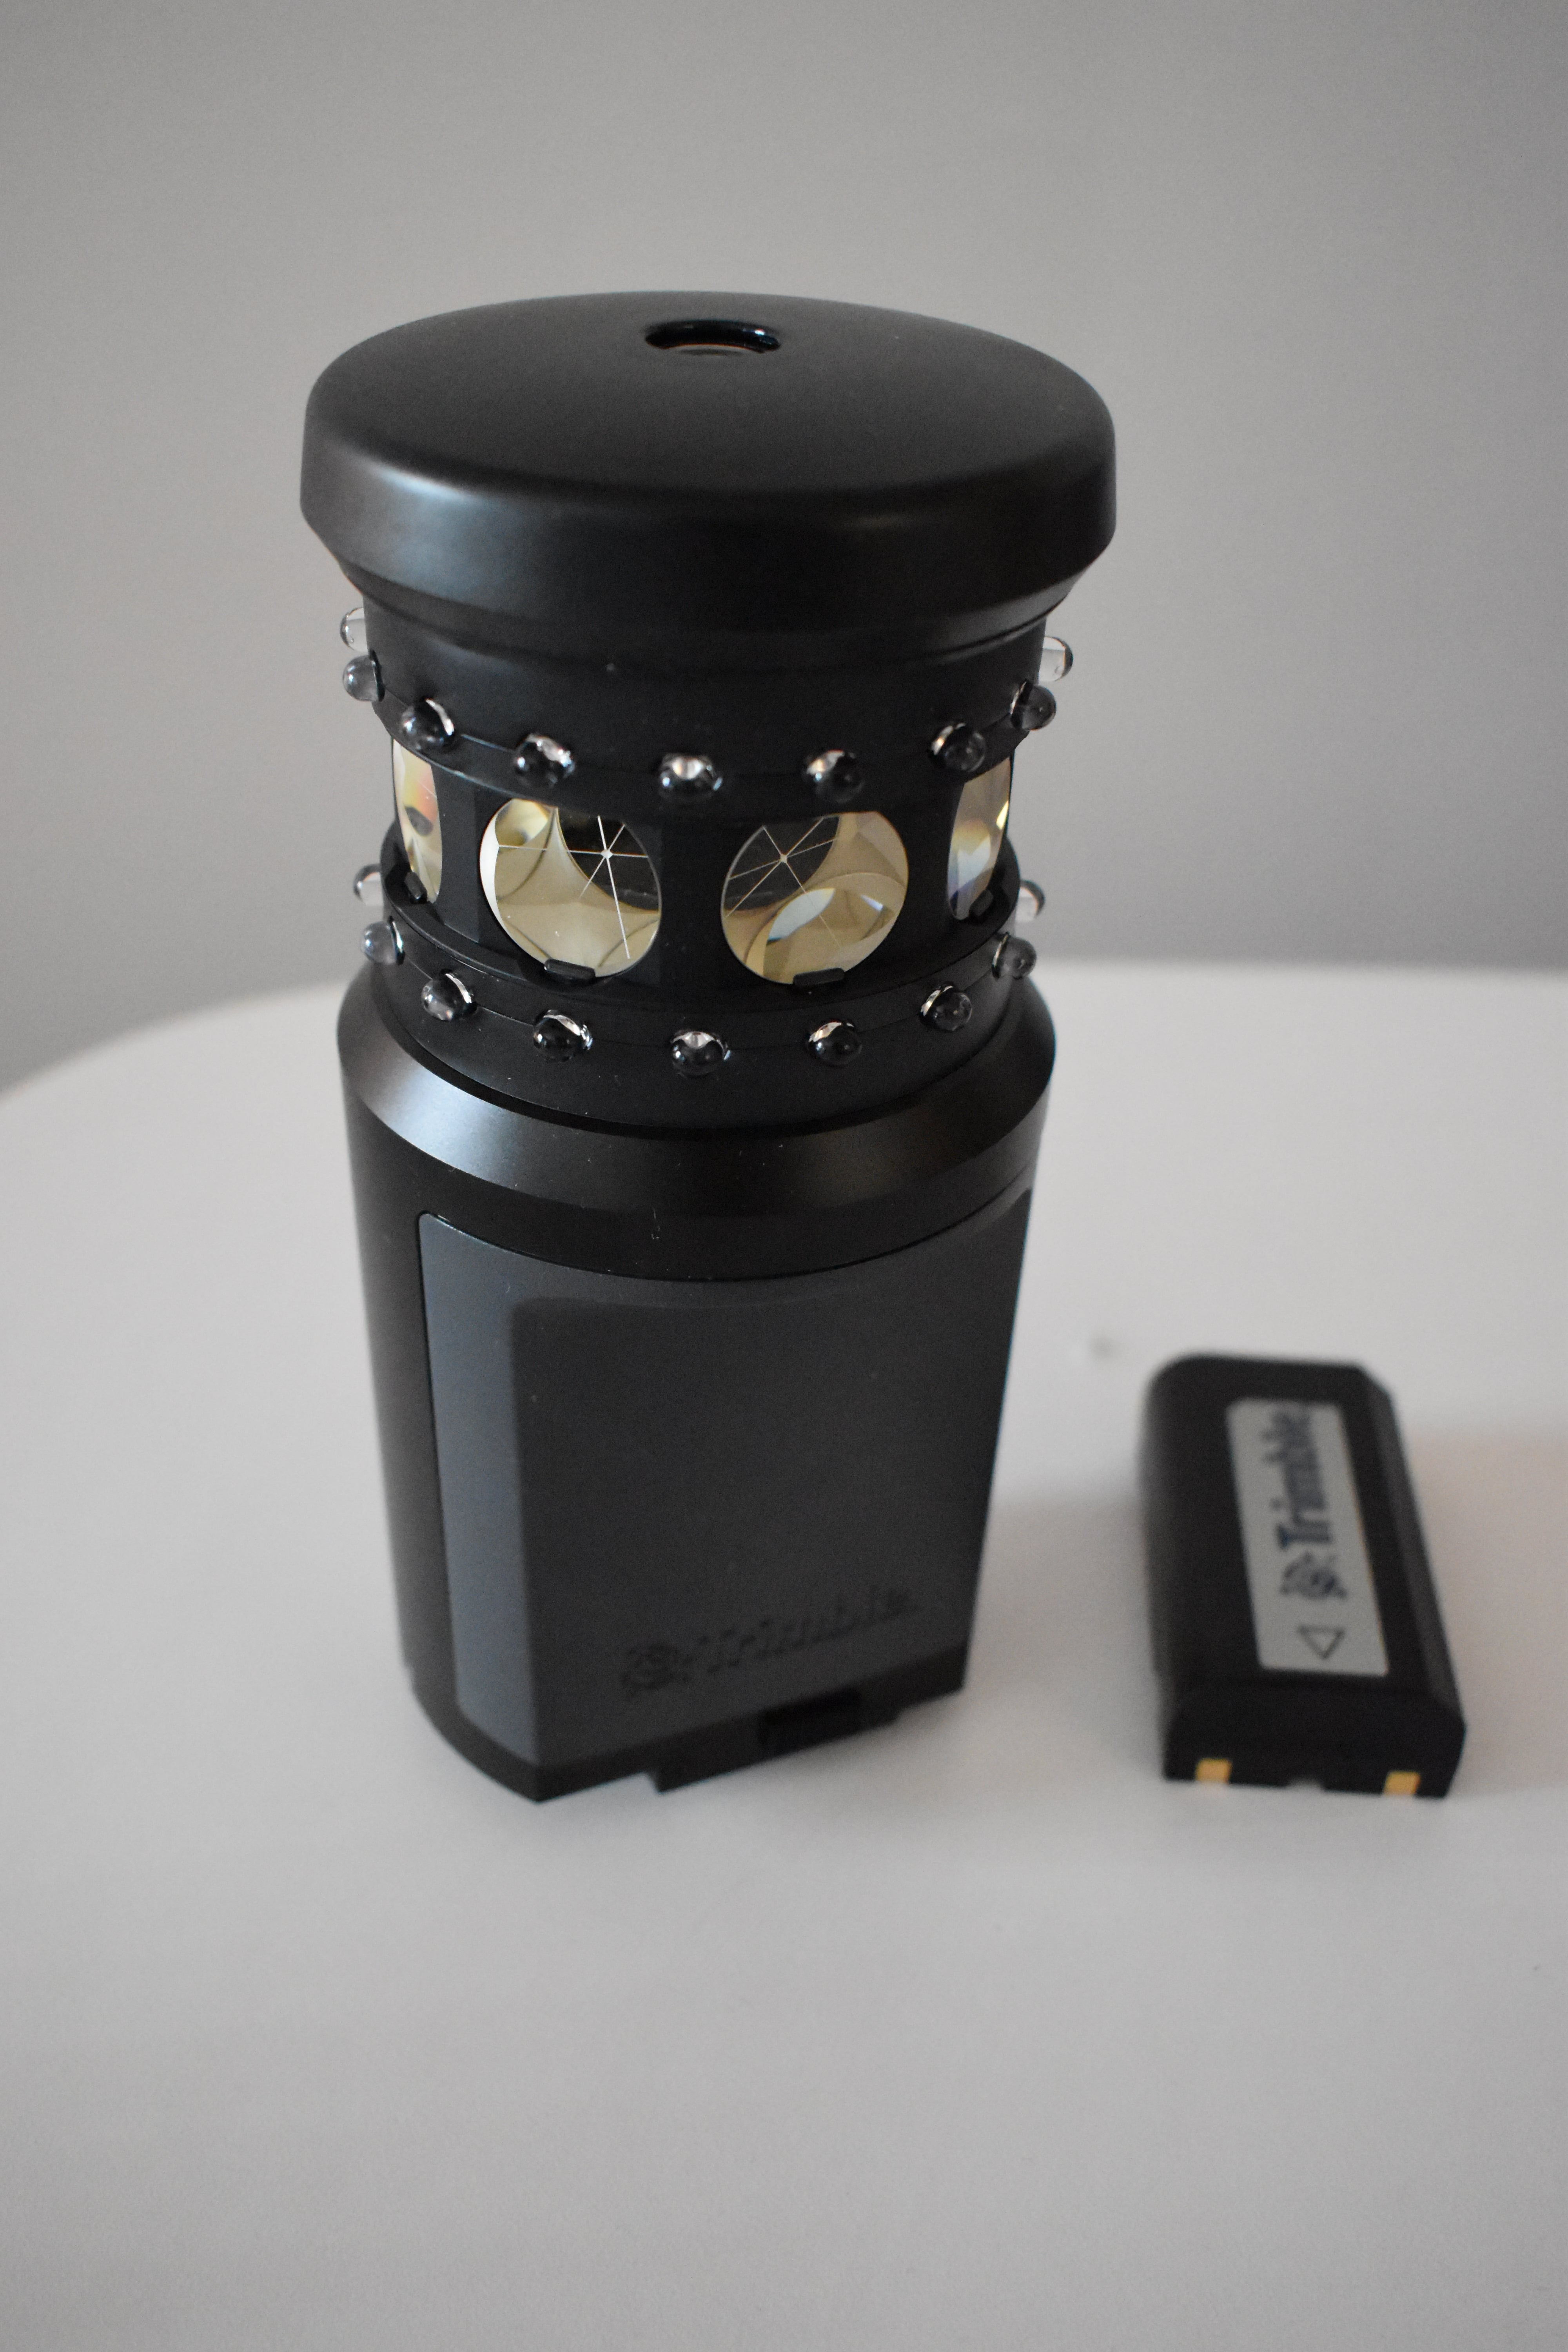
\includegraphics[width=0.2\textwidth]{./figs/prism.JPG}
	\caption{Prism used as target with trimble S7.}
	\label{fig:prism}
\end{figure}

Ce prisme a de nombreux atout.
Premièrement, il est possible de demander à un théodolite de se verrouiller sur celui-ci.
Le théodolite ne changera pas de cible durant la prise de mesure.
Le prisme contient une signature numérique unique qui garantie ce verrouillage.
Cela permet de placer plusieurs prismes sur une même plateforme robotique tout en garantissant la bonne prise des mesures.
De plus, les performances des mesures sont augmentées.
Il est possible de suivre le prisme sur de plus longues distances avec une précisions accrues.
Enfin, il est possible de le fixer solidement à une plateforme via une vis.
Le prisme fonctionne avec une batterie qui permet d'activer sa signature électronique. 
Il est possible de régler le numéro de cette signature (allant de 1 à 8) afin de le différencier d'autres prismes.
Cette cible est assez lourde et onéreuse.
Lors de son utilisation, il convient donc d'en prendre soin et de l'utiliser de manière sécuritaire pour éviter de l'endommager.
Une notice papier est fourni avec l'équipement, illustrant son utilisation et les précautions à prendre.

\subsection{Communication part}

La communication des données vers une plateforme robotique devient difficile avec les équipements fournit avec le théodolite.
L'USB ou le Bluetooth ne sont pas adapté, tandis que le relai n'est utilisable que sous l'application Trimble Access qui fonctionne sur Windows exclusivement.
Nous avons décidé d'utiliser un autre module de communication pour résoudre ce problème.
Il s'agit d'un module de communication par antenne LoRa sur un circuit imprimé que l'on peut configurer pour transmettre des données sur de longues portées.
Ce module sera installé sur une carte Raspeberry Pi 3B+, qui recevra les données du théodolite par USB.
La plateforme robotique sera équipée également d'une Raspberry Pi 3B+ et d'un module LoRa pour communiquer avec le théodolite, ce qui nous permettra de sauvegarder les données à distance.

Le module LoRa est présenté à \autoref{fig:LORA}.

\begin{figure}[htb]
	\centering
	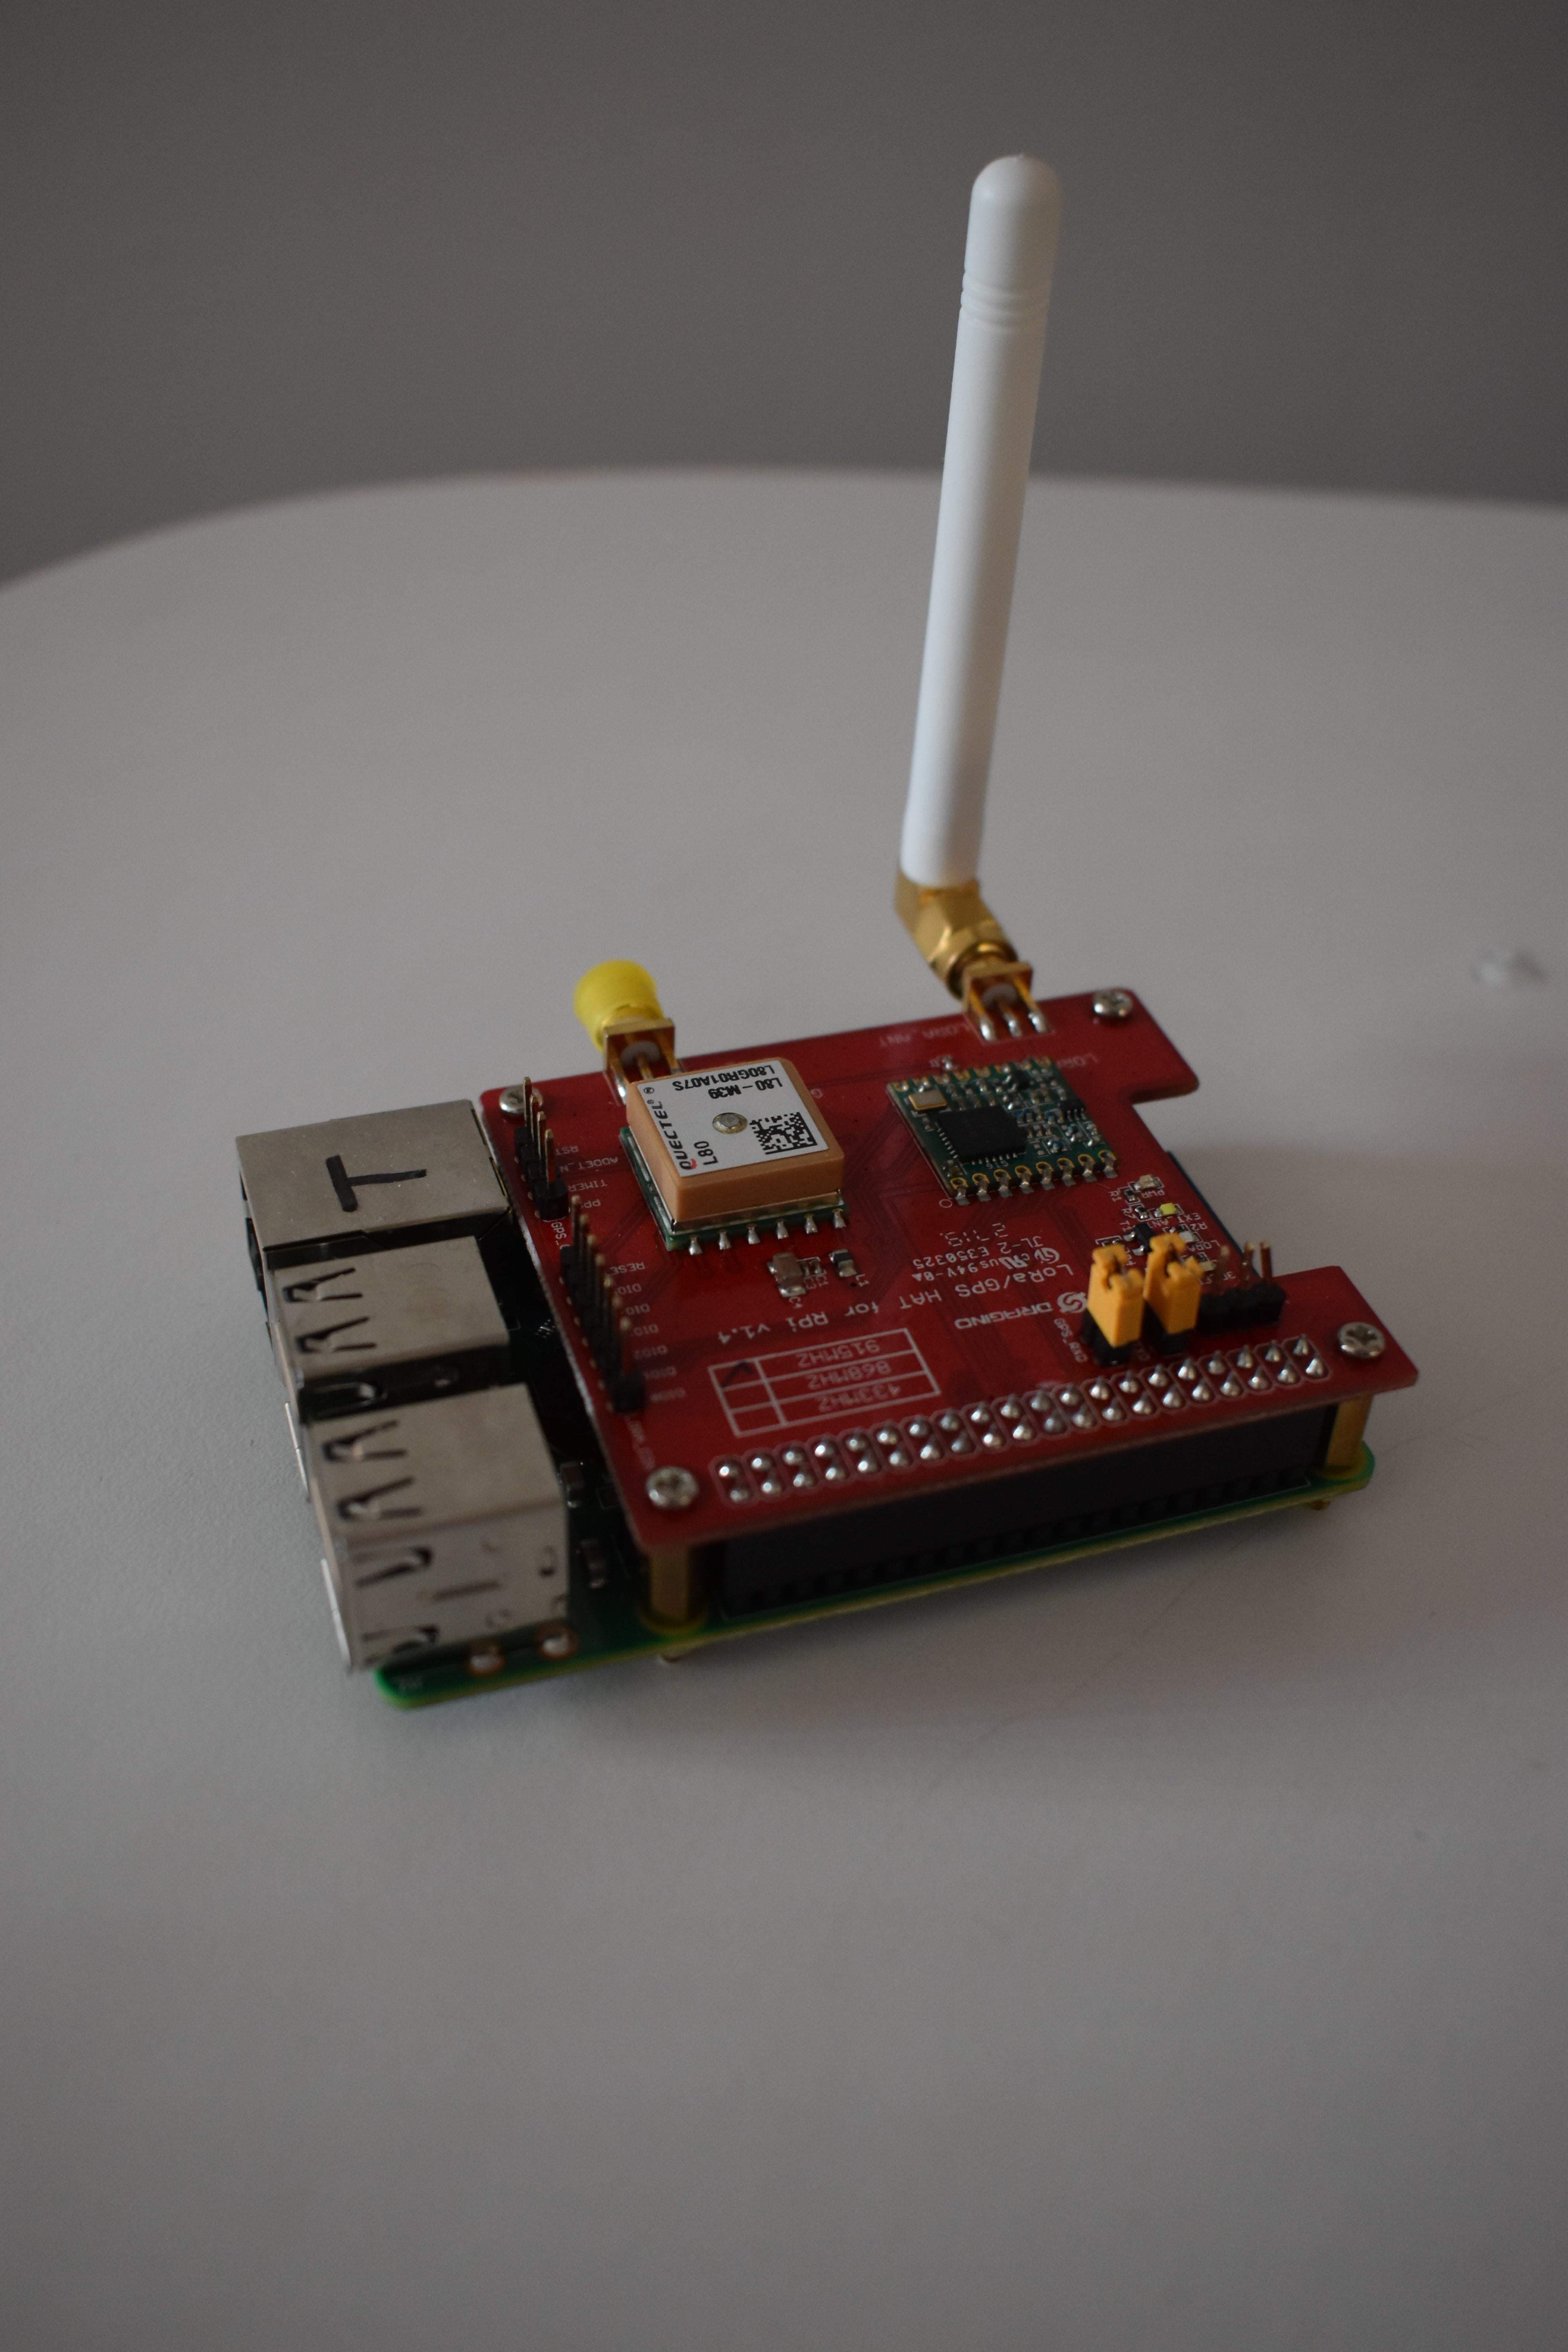
\includegraphics[width=0.2\textwidth]{./figs/LoRa_antenna.JPG}
	\caption{LoRa antenna and it shield used on a Rspberry Pi 3B+.}
	\label{fig:LORA}
\end{figure}

\href{https://wiki.dragino.com/index.php?title=Lora/GPS_HAT}{Ce site internet} donne une vue d'ensemble des possibilités qu'offre ce module, ainsi que quelques exemples de codes pour certaines applications.

Le document suivant \href{run:LoRa_GPS_HAT_manual.pdf}{LoRa GPS HAT Manual} donne des exemples plus détaillé d'utilisation, ainsi qu'un guide de démarrage pour celles-ci.
Des informations complémentaires seront données dans la \autoref{ROS_node} et \autoref{Deployment}.

\subsection{Raspberry Pi 3B+}

The computer currently used to interface with the theodolite is a Raspberry Pi 3 model B+ running Ubuntu Mate 18.04.2. 
Using another computer and operating system should theoratically work, as long as the OS is a Linux distribution and as long as the computer has a 32-bit ARM based processor. 
The only computers that have been tested are Raspberry Pi 3 model B/B+ and the only OS's that have been tested are Ubuntu Mate 18.04.2 and Raspbian 9.11 Stretch.

The credentials for logging in the computer are the following:

\begin{itemize}
    \item User: pi
    \item Password: macaroni
\end{itemize}


% -------------------------------------------------------------
\section{Software}
\label{sec:software}

La configuration du théodolite peut se faire de deux manières différentes.
La plus pratique et la plus rapide à mettre en œuvre consiste à utiliser l'application Trimble Access.
Cette application est uniquement disponible sur Windows, mais permet d'utiliser toutes les fonctionnalités du théodolite assez rapidement.
Le second moyen est d'utiliser des librairies C++ de code qui permettent de communiquer avec le théodolite.
Ces librairies peuvent être utilisées sous Linux, mais ne contiennent pas toutes les fonctionnalités possibles sous Trimble Access.
De plus il est difficile de mettre en œuvre celle-ci dans certains cas.
Cette section présente ces différents moyens de configurer le théodolite.

\subsection{Trimble Access software (coming soon)}

Description des possibilité offertes par le logiciel de Trimble
Détailler et montrer les fonctionnalités les plus couramment utilisées

\subsection{Compile library for linux}

L'entreprise Cansel nous a fournit des librairies pré-compilées de code C++ permettant d'utiliser certaines fonctionnalités du théodolite sous Linux.

This repository is built upon a project that was intended to be used as a Telnet server for interfacing with a Trimble TotalStation robotic theodolite. 
Its main program was modified heavily by removing the telnet server functionnality and replacing it with a sequence of simple commands that are sent to the theodolite. 
This was done in order to test and explore what type of interfacing could be done with the theodolites we have at the lab, which are 3 Trimble TotalStation S7. 
In other words, the main program now consists of a small sequence of commands that are sent to the theodolite before terminating.

Dans le package theodolite\_node\_ROS, ces librairies se trouvent dans le répertoire $lib$.
Les fichiers d'entêtes $.h$ qui utilisent ses librairies sont dans le répertoire $include$.
Pour utiliser ces librairies pré-compilées, des fichiers $.cpp$ et $.h$ ont été créés dans le répertoire $src$.
Ces fichiers sont issues d'un SDK fournit par Trimble.
Nous détaillerons celui-ci dans les sous-sections à venir.
Les fonctions définit dans ces fichiers seront explicités, principalement celles que nous utilisons pour obtenir les données du théodolite.
Les deux principales classes que nous allons utiliser sont ObservationListener et SsiInstrument, présent dans le répertoire $src$.

\subsubsection{TPSDK}

The main program can access the functionnalities of the theodolite through the use of the Trimble Precision SDK (TPSDK). 
This SDK is provided by the manufacturer of the theodolite in order to allow the theodolite to be integrated into 3rd party software solution.

The SDK is made to be used with Win32 and Windows Mobile platforms. 
However, this repo uses a special non-official precompiled version of this SDK that is meant to be used on a Raspberry Pi running Raspbian. 
In our case, the SDK consists of .so library files and .h header files, that are located in the lib and include directories, respectively. 
The source code in this repo is written in C++. 
The main program, which has dependencies to the SDK, has been compiled and used on a Raspberry Pi 3 model B+ running both Raspbian 9.11 Stretch and Ubuntu Mate 18.04.2.

More detailed explanations and description of the SDK are available on the TPSDK website. 
To sign in, click Sign In to Trimble Access and enter the following info:

\begin{itemize}
	\item Username: ULaval
    \item Organization: trimble-precision-sdk
    \item Password: ulav123!
\end{itemize}    

On this website you will find a complete description of the SDK, as well as guides and lists of features that are accessible with the SDK. 
More importantly, you will find the list of the classes in the SDK, along with their methods, attributes and interfaces. 
It is important to know that the documentation on this website may not correspond exactly to the version used in this repo, since we use a C++ ARM based version of the SDK, instead of the Microsoft .NET version. 
For this reason, the interfaces might not be the same and they might not be directly usable via C++.
Also, since we are not sure about where our version of the SDK is situated in the version release history, some features described in the documentation may not be available in our version of the SDK.

\subsubsection{Communication}

The Trimble TotalStation SSeries supports many type of communication channels, such as Bluetooth, radio, serial, USB, WiFi, etc. 
However, we were not able able to connect the Raspberry Pi to the TotalStation S7 via Bluetooth or WiFi. 
The lab has in its possession three Trimble TDL2.4 data link radios, which connect to a computer via Bluetooth and connect to a theodolite via 2.4 GHz radio channel. 
They could prove usefull for long distance communication between the Raspberry Pi and the theodolite, but we have not been able yet to connect them to a Raspberry Pi and use them. 
They currently only work with the tablet controller of the theodolite.

This repo currently only supports communication between the Raspberry Pi and the theodolite via a USB and TCP connection. 
The theodolite shows up in Linux as a USB device with idProduct: 0101, idVendor: 099e and Trimble as manufacturer. 
A udev rule was created in Ubuntu Mate in order to give users access to the theodolite USB connection.
Any user in the group users can run the program and communicate with the device. 
The TCP connection that was already implemented has not been used or tested.

Since the SDK was made to be used on Windows, the default classes for instanciating a communication channel with the theodolite don't work on Linux. 
The SDK supports custom communication type, as long as you define a custom communication class which inherits from ICommunicator and implements the methods defined in the ICommunicator interface.
The classes USBCommunicator and TCPCommunicator are two implementation of this interface. They are used in the SsiInstrument class in the Connect method.

\subsubsection{SsiInstrument}

The class SsiInstrument represents the TotalStation theodolite at a high level of abstraction. 
It implements methods that start specific tasks with a few number of parameters. 
These methods handle the required sequence of function calls specific to the SDK.

In order to use the features that are implemented in the SsiInstrument class and start interfacing with the theodolite, one must first instantiate an SsiInstrument object and load the appropriate driver. 
The default loaded driver is a driver for the TotalStation SSeries theodolites. 
The method to call is SsiInstrument::LoadDriver. 
It essentially instantiates the appropriate device driver from its DriverManager attribute, which is instantiated in the initialisation list in the constructor of the class. 
The driver is an SSI::IDriver object that is kept as an attribute of the class.

When the driver is loaded, the SsiInstrument::Connect should be called in order to establish a connection to the device. 
Two parameters can be passed to this function: const char* sType and const char* sPort. 
The sType parameter specifies the type of communication channel to use. 
The following types can be specified: "usb", "tcp" and "int". 
The USB and TCP types use the previously mentionned implementations of the ICommunicator interface: USBCommunicator and TCPCommunicator. 
USBCommunicator uses the external library libusb-1.0 to connect to the device. 
The int type of connection stands for internal. 
It is not clear what this type of connection means and connecting to the device with this type of connection hasn't been tested. 
The parameter sPort is used to specify the TCP port to be used if the type of connection is TCP.
Again, this type of connection has also not been tested. 
According to the user manual, the TotatStation S7 doesn't seem to support connection via an IP network. 
The SsiInstrument::Connect method instantiates a SSI::ISensor object and keeps it as an attribute of the class that can be used to access interfaces.

Once the driver is loaded and the device is connected, the user can now call functions to interface with the device. 
Basic features such as starting video streaming, taking measures, tracking targets and setting the servos angles have been implemented.

In order to access an intrument feature, the SSI::ISensor::getInterface method of the SSI::ISensor object (\_pSensor attribute) has to be called while passing it the interface of the feature you want to access. 
Once you have the interface, you can call the methods defined by the interface to start interacting with the device. 
Documentation for the interfaces is available on the TPSDK website.

Plusieurs mode de tracking sont définis dans la classe SsiInstrument. 
Il s'agit des modes: MODE\_PRISM, MODE\_AUTOLOCK, MODE\_DR, MODE\_DR\_LASER et MODE\_MULTITRACK.
MODE\_PRISM permet de trouver un prisme pour effectuer une mesure par la suite.
MODE\_AUTOLOCK fait en sorte que le théodolite se verrouille sur une cible dès qu'il la trouve, et peut changer de cible s'il en trouve une autre. 
C'est un mode de suivi sans prise de mesure.
MODE\_DR permet de ce verrouiller sur une cible et d'effectuer une mesure uniquement.
MODE\_DR\_LASER effectue la même tâche que MODE\_DR, mais en plus un puissant rayon laser est utilisé afin de visualiser la zone de prise de mesure.
Enfin, MODE\_MULTITRACK permet au théodolite de se verrouiller sur un prisme et d'effectuer un suivi de celui-ci tout en prenant des mesures à une fréquence pré-défini.
C'est ce mode que nous allons utiliser pour prendre des références de trajectoires.

Pour activer un mode, on utilise la fonction $Target$.
Cette fonction prend en entrée le mode choisit, ainsi que le numéro de la cible qui est dans notre cas le numéro du prisme que l'on a sélectionné.
Par la suite, le tracking est activé par la fonction $Tracking$ qui prend en argument l'information démarré/arrêté, et un objet de la classe ObservationListener pour sauvegarder les données de positionnement.
Une fois le tracking activé, les données reçues sont automatiquement stockées dans cette classe.
Pour y avoir accès, il suffit d'utiliser les fonctions de la classe ObservationListener.

\subsubsection{ObservationListener}

This class is one of the most important for our usage.
It define a vector element which will contain all the data gather.
This vector is named $observations$, and his size is defined as $size_vector$.
The function $getObservations$ and $getSizeVector$ will be used several times to have access to the data.

The index of the vector $observations$ is defined by an enumeration list.
Five topics are listed: HORIZONTAL\_ANGLE\_VECTOR, VERTICAL\_ANGLE\_VECTOR, DISTANCE\_VECTOR, TIMESTAMP\_VECTOR and ERROR.
These topics are updated in the function $observationTracked$.
This function monitors an event of the theodolite and save the data received.
The two first one are the data of horizontale angle and verticale angle of the trimble.
These data are expressed in arc-second unit, cast into a double for an easier storage.
The DISTANCE\_VECTOR expresses the distance of the measurments in meter.
If the target is not detected or too close to the trimble, the value will be zero.
The timestamps are stored in TIMESTAMP\_VECTOR.
These data used UTC time as timestamps, so it will be the clock of the computer.
The time is expresses as a double.
The frequency of the measurement will depend of the configuration choose for the tracking.
Finally, ERROR is a flag which will tell the user if there are some issues to collect the data.
The different flags are presented is the Table ...

%%Table flag
%%%%%%%%%%%%%%%%%%%%%%%%%%%%%%%
%%%%%%%%%%%%%%%%%%%%%%%%%%%%%%%
%%%%%%%%%%%%%%%%%%%%%%%%%%%%%%%
%%%%%%%%%%%%%%%%%%%%%%%%%%%%%%%
%%%%%%%%%%%%%%%%%%%%%%%%%%%%%%%
%%%%%%%%%%%%%%%%%%%%%%%%%%%%%%%

If the user choose a finite number of measurements, he can use the function $saveFile$ to store the data in a CSV file.

\subsubsection{Others class functions}

Les autres classes présent dans le répertoire $src$ ne sont pas utilisées actuellement, ou permettent de faire appliquer les fonctions des deux classes précédentes.
Il s'agit de SsiCallbacks, SsiCommand, TCPCommunicator, TCPServer, USBCommunicator et
VideoStreamingListener.
SsiCallbacks possèdent des fonctions qui permettent l'état de certaines configurations.
Par exemple l'on peut demander à connaître le tilt du théodolite ou si le tracking est toujours en cours.
SsiCommand est une classe qui permet d'envoyer les commandes demandées au théodolite (par exemple $connect$ ou $target$ entre-autres).
TCPCommunicator et TCPServer sont des classes qui nous autorisent à communiquer avec le théodolite par liaison TCP.
Nous ne les utiliserons pas dans ce projet.
USBCommunicator nous permet de communiquer par USB avec le théodolite.
Enfin, VideoStreamingListener est une classe qui possèdent des fonctions pouvant utiliser la caméra du théodolite.
Nous ne l'utiliserons pas également dans ce projet.

\subsubsection{Remark}

L'utilisation de la librairie C++ ne peut pas se faire en même temps que l'utilisation du logiciel Trimble Access.
EN effet, dès que l'un ou l'autre des logiciels est démarré, le port USB est occupé et ne peut pas se connecter à d'autres programme pour recevoir des informations autres que celles demandées par le logiciel utilisé.
De ce fait, il convient d'utiliser dans un premier le logiciel Trimble Access pour calibrer et configurer la plateforme comme on le souhaite.
Par la suite, le programme sous linux nous fournira les données acquissent.

Some features require receiving data asynchronously from the device. 
Methods like SsiInstrument::Video and SsiInstrument::Tracking require passing listeners that are classes that inherit and implement specific interfaces. 
For example, in order to access the video streaming frames and the streaming states when calling the SsiInstrument::Video method, one has to pass an object that implements SSI::IVideoStreamingUpdateListener and SSI::IStreamingStateChangedListener. 
The methods defined by these interfaces are called whenever an event happens. 
Data is accessible in an event object (such as SSI::VideoStreamingUpdateEvent) that is passed as parameter in the callbacks defined in the interface.

In our case, two listeners have been developped in order to be able to access tracking measures and video streaming frames. 
These listener are ObservationListener and VideoStreamingListener respectively. 
All they currently do is store the current image or store the received measurements in a vector. 
It is also possible to save the received measurements to a .csv file.
Initially, the repo came with the SsiCallbacks class. 
This class implemented some listeners that were usefull with the Telnet server that was implemented.
All of these library are compiled under ROS to parameter the code we want to use.
The next section is about two nodes we have made: one to send the data through LoRa antenna, and one to receive these data again through LoRa antenna.

% -------------------------------------------------------------
\section{ROS node}
\label{ROS_node}

ROS (Robot Operating System) est très utilisé en robotique.
C'est une méta-librairies qui contient des packages de code pouvant être utilisés sur différentes plateformes, principalement sous Linux.
Cette librairie permet de lancer des nœuds de code pouvant communiquer des informations entre eux à travers des publisher et subscriber.
Afin de pouvoir paramétrer plus facilement notre code pour récupérer les données du théodolite, nous utiliserons un nœud de ROS qui aura pour but d'envoyer les données via les antennes LoRa, et un autre nœud de ROS qui les réceptionnera pour les enregistrer sur la plateforme robotique.
Cette section décrira le fonctionnement de ces deux nœuds.
Le package qui contient ces deux nœuds est nommé theodolite\_node\_ROS.

\subsection{Acquisition of data and sender}

Dans le package theodolite\_node\_ROS et dans le répertoire $src$, se situe le nœud de ROS qui permet d'envoyer les données du théodolite vers l'antenne LoRa réceptrice.
Le fichier correspondant est nommé $theodolite_node.cpp$.
Les différents paramètres de la communication avec l'antenne LoRa ainsi que les fonctions utilisées avec celle-ci sont définies juste avant la principale fonction $main$.
Cette fonction $main$ se compose d'une boucle while qui effectuera plusieurs tâche à la suite.

Tout d'abord on récupère les paramètres de la configuration que l'on souhaite.
Ces paramètres sont définis dans le launchfile $theodolite\_node.launch$ présent dans le répertoire $launch$ du package.
Six paramètres peuvent être définit.
Il faut dans une premier renseigner le numéro du théodolite ($theodolite\_number$) que l'on souhaite utiliser.
Ce numéro, c'est nous qui le choisissons.
Il doit être différent des autres théodolites utilisés s'il y en a plusieurs.
Ce numéro servira à trier les données récoltées, notamment dans le cas où plusieurs théodolite track la même cible.
Le numéro doit être compris entre 1 et 8 inclus.
Ensuite il faut donner le numéro du prisme que l'on souhaite traquer, $target\_prism$.
Ce numéro servira également lors du tri des données.
Le troisième paramètre, $number\_of\_measurments$, à renseigner est le nombre de mesures que l'on souhaite effectuer.
Si l'on veut faire une prise de mesure continue dans le temps, on doit mettre la valeur de 0.
Le programme ira alors chercher les données à chaque fois qu'une nouvelle apparaît.
L'utilisateur devra alors fermer le noeud manuellement via le terminal.
Le paramètre $use\_lora$ indique au programme si l'on veut envoyer les données via les antennes LoRa.
Le paramètre $show\_data$ peut être utilisé pour debugger en affichant les données reçues du théodolite sur le terminal.
Enfin, il est possible de sauvegarder un nombre de donnée finis grâce aux paramètres $save\_measurements$ et $file\_measurements$, qui indiquent respectivement si l'on veut sauvegarder les données ainsi que le nom du fichier si c'est le cas.
Il est à noté que pour sauvegarder des données, le paramètre $number\_of\_measurments$ doit être différent de 0.
De plus, seul le format $.csv$ est utilisé.

Le code exécute par la suite les fonctions d'initialisation de l'antenne LoRa si l'option est activée.
Un contrôle des valeurs des paramètres est ensuite effectué pour s'assurer qu'il n'y a pas d'erreurs.
Les drivers du théodolite sont ensuite chargés avec la fonction $LoadDriver$, et la connexion est activée par la fonction $Connect$.
S'il n'y a pas d'erreur à ce niveau, on donne le mode de tracking au théodolite via la fonction $Target$.
Ensuite on définit notre vector $observation_listener$ qui contiendra les données reçues du théodolite.
Le tracking avec la prise de données débute avec l'appel de la fonction $Tracking$.
Le code se divise en deux parties: une partie pour la prise de mesure en continue, et une autre qui effectue un nombre donné de mesures.

Si la prise de mesure est continue, on utilise une boucle while sans fin afin d'acquérir les données.
Le nombre de données dans notre vector $observation_listener$ est alors contrôlé régulièrement afin de détecter si de nouvelles valeurs ont été enregistrées.
Une pause de 30 millisecondes est effectuée entre chaque contrôle afin de laisser le temps au programme de se mettre à jour.
Ce délai est plus petit que la fréquence maximale théorique à laquelle le théodolite peut transmettre des données (20Hz).
De ce fait, le programme ne manquera pas de nouvelles données.
Lors de la détection de nouvelles données, celles-ci sont accessible via notre vector.
Lorsque l'option $show\_data$ est activée, les valeurs sont affichées sur le terminal.
SI $use\_lora$ est activé, les données sont castées dans une variable de type string, puis envoyé byte par byte à l'antenne LoRa qui les diffusera.
Pour une prise de mesure finie, la même procédure est appliqué, si ce n'est que la boucle while se termine quand le nombre de mesures voulue est atteint.
Après que ce nombre soit atteint, le programme sauvegarde les données si l'utilisateur a activé l'option, puis le nœud de ROS se déconnecte du théodolite avec la fonction $FreeDriver$.

Il y a 7 données qui sont envoyées lors de la communication avec la plateforme robotique.
La première valeur est le numéro du théodolite, suivi par le numéro du prisme afin de différentier plus type de mesure entre-elles.
Ensuite les mesures angulaires sont envoyées: l'angle horizontale et l'angle verticale.
La distance par rapport au prisme est la 5ème donnée envoyée, suivi du timestamp des mesures angulaires et de la distance.
Enfin, un flag des erreurs définit à la \autoref{sec:software} est envoyé en dernier dans la chaîne de caractère.

IL est possible que des erreurs de connexion ou autres se produisent durant le déroulement du programme.
La \autoref{sec:issue} y est consacrée, et apporte des solutions pour résoudre les problèmes survenus.
Maintenant que nous pouvons envoyer les données, le code pour les recevoir est décrit dans la sous-section suivante.

\subsection{Receiver}

Comme le précédent noeud de ROS, le noeud d'écoute des données se situe dans le package theodolite\_node\_ROS et dans le répertoire $src$.
Le fichier correspondant est nommé $theodolite\_listener.cpp$.
Les différents paramètres de la communication avec l'antenne LoRa ainsi que les fonctions utilisées avec celle-ci sont définies juste avant la principale fonction $main$.
Cette fonction $main$ se compose également d'une boucle while qui effectuera plusieurs tâche à la suite.

Tout d'abord on récupère les paramètres de la configuration que l'on souhaite.
Ces paramètres sont définis dans le launchfile $theodolite\_listener.launch$ présent dans le répertoire $launch$ du package.
Deux paramètres y sont utilisés.
Le premier paramètres, $rate$, sert à définir la fréquence de l'écoute de la réception des messages.
Le second paramètre $show\_data$ sert à afficher les données reçues sur un terminal afin de debugger ou vérifier que la communication fonctionne correctement.
Une fois que les paramètres ont été définit, l'antenne LoRa est configuré comme pour le code de l'émetteur.
La différence est que l'on utilise une boucle while sans fin, dans le but d'écouter en tout temps la réception d'un message à la fréquence définie par l'utilisateur.

Cette boucle while sans fin exécute la fonction $receivepacket$, fonction qui va lire les bytes reçus et les convertir au format double.
Les données reçues sont ensuite sauvegarder dans un vector qui sera transmit sur ROS pour un publisher nommé $data\_publish$.
Par la suite, il suffit de sauvegarder ces données dans un rosbag pour pouvoir les utiliser en post-traitement.
Il est à noté que ce publisher n'utilise pas de timestamp de ROS.
En effet, il est trop compliqué de synchroniser les données issues du théodolite avec l'horloge de ROS en temps réel.
Cette synchronisation devra se faire en post-traitement.
De plus, ce code ne fonctionne pour le moment que pour une seule communication émetteur-récepteur.
Des tests devront être effectués pour le valider avec plusieurs émetteurs vers un récepteur.

% -------------------------------------------------------------
\section{Deployment (Coming soon)}
\label{Deployment}

Courte introduction pour le déploiement de différents theodolite

\subsection{Calibration of theodolite}

Mise en place sur trépied \\
Réglage du tilt \\
Autres ? \\

\subsection{Resection}

Pourquoi ?
Comment définir le repère du theodolite avec une/plusieurs cibles \\
Si pas de prism ? \\

\subsection{ROS node receiver}

Mise en marche du code pour le receiver

\subsection{ROS node sender}

Mise en marche du code pour le sender

% -------------------------------------------------------------
\section{Issue/error (Coming soon)}
\label{sec:issue}

Table des erreurs pouvant survenir durant le déploiement et les solutions à apporter

% ---------------------------------------------------------------
\printbibliography


\end{document}
